\documentclass[promaster,eversion]{thesis-guet} 
% eversion:电子版 pversion:打印版 bachelor:本科 master:学硕 promaster:专硕 doctor:博士 
% latex基础教程 lshort-zh
% \usepackage{showframe} % 显示排版框架
\usepackage{color, framed} % 高亮显示
\definecolor{shadecolor}{RGB}{255,204,75} % 定义高亮颜色
\secrets{绝密} % 不涉密请注释该命令,不要空着
\title{基于嵌入式散热模块的微通道散热技术研究}{Research on microchannel heat dissipation technology based on embedded heat dissipation module}
\author{李雪斌}
\advisor{李XX} % 导师姓名
\protitle{教授} %导师职称
\school{机电工程学院}
\major{机械工程}
\studentnumber{2020XXXXX}
\degreecategories{工学硕士}
\datereply{\today} % 可更换为具体日期如:\datereply{2023年5月28日}

\graphicspath{{./picture/},{./picture/Chapter1/},{./picture/Chapter2/},{./picture/Chapter3/},{./picture/Chapter4/},{./picture/Chapter5/}} % 图片所在位置


%%全文开始
\begin{document}
    \makecover % 封面
    
    % % \bindpdfcover{PDF文件} % 可使用封面PDF文件,如盲审封面
    % \originalitydeclaration % 独创性声明
    % % \signatureofdeclaration{PDF文件} % 可使用已签字的独创性声明PDF文件
    % % !Mode:: "TeX:UTF-8"


\begin{chineseabstract}
    随着人工智能和第五代移动通信技术的发展,推动着电子芯片向着小型化和高集成化的方向快速发展的同时也导致电子芯片的发热问题日益严重。
    电子器件55\%的故障是由温度引起,而在温度引起的故障问题中有很大一部分是由温度分布不均而引起的。
    因此,在为芯片散热的过程中,不仅要考虑热源的最高温度,还要考虑整个热源温度分布的均匀性。
……

\chinesekeyword{微通道;嵌入式散热模块;多目标优化;NSGA-Ⅱ;多热源散热}
\end{chineseabstract}

\begin{englishabstract}
    With the development of artificial intelligence and fifth-generation mobile communication technology, electronic chips are developing rapidly towards miniaturization and high integration, but the heating problem of electronic chips is becoming more and more serious.
    55 percent of the faults in electronic devices are caused by temperature, and a large part of the fault problems caused by temperature are caused by uneven temperature distribution.

\englishkeyword{Microchannel; embedded heat dissipation module; Multi-objective optimization; NSGA-Ⅱ; Multi-heat source heat dissipation}
\end{englishabstract}% 摘要
    % \thesisfigurelist % 插图目录
    % \thesistablelist % 插表目录
    % \thesissymbollist %符号说明表
    % \thesistableofcontents % 目录

    % % A组表示希腊字符说明,B组为下标说明,C组为缩略词说明。
\nomenclature[C,01]{PCB}{Printed Circuit Board}
\nomenclature[C,02]{LTCC}{Low temperature cofired ceramic}
\nomenclature[C,03]{MATD}{mean absolute temperature deviation}

\nomenclature[]{$T_{f}$}{流体温度 $(K)$}
\nomenclature[]{$T_{s}$}{固体温度 $(K)$}

\nomenclature[A]{$\rho_{f}$}{流体密度 $(kg/m^3)$}
\nomenclature[A]{$\mu_{f}$}{流体动力粘度 $(kg/(m \cdot s))$}

\nomenclature[B]{$s$}{固体}
\nomenclature[B]{$f$}{流体}
% \nomenclature[B]{$$}{}       % 符号定义文件
    % % 引用各个章节的文件
    % % !Mode:: "TeX:UTF-8"
%此为第一章节。
%\figure为图片,[h]为hear代码所在,\caption为表名图名,\includegraphics为引用位置,\cite为引用参考文献,\begin{equation}公式,\subfloat子图,\label标签,\begin{table}表格,\begin{tabular}三线表,{cccc}完全居中,\toprule,\multirow取几行,\cmidrule取第几列\begin{theorem}定理,\begin{proof}证明,\begin{corollary}推论,\begin{lemma}引理
    
\chapter{绪\quad 论}
\section{研究工作的背景与意义}

\begin{shaded}
    微电子器件整体发展趋势  
    \end{shaded}
    随着人工智能和第五代移动通信技术等系统技术的发展,推动着半导体行业在移动便携设备、高性能计算机、自动驾驶、物联\cite{lau_recent_2022}网和大数据等应用领域的发展\cite{lau_recent_2022},同时也推动着电子芯片向着小型化和高集成化方向发展快速发展\cite{sadique_heat_2022}。在过去的几十年里处理器上的晶体管数量依照这摩尔定律\cite{moore_cramming_1965}的预测呈现出指数级的增长趋势,如\cref{chip-develop}所示。摩尔定律与登纳德定律\cite{dennard_design_1974}引领着半导体行业飞速发展,半导体芯片上电子元件的数量与日俱增,大大提高了芯片的综合性能。随着半导体芯片性能的提高,以及尺寸的限制,导致芯片工作时温度的急剧上升,这将对其正常的运行工作产生严重的影响。半导体芯片散热器技术的发展已成为制约半导体芯片进一步发展的一大重要原因。

    \begin{figure}[h]
        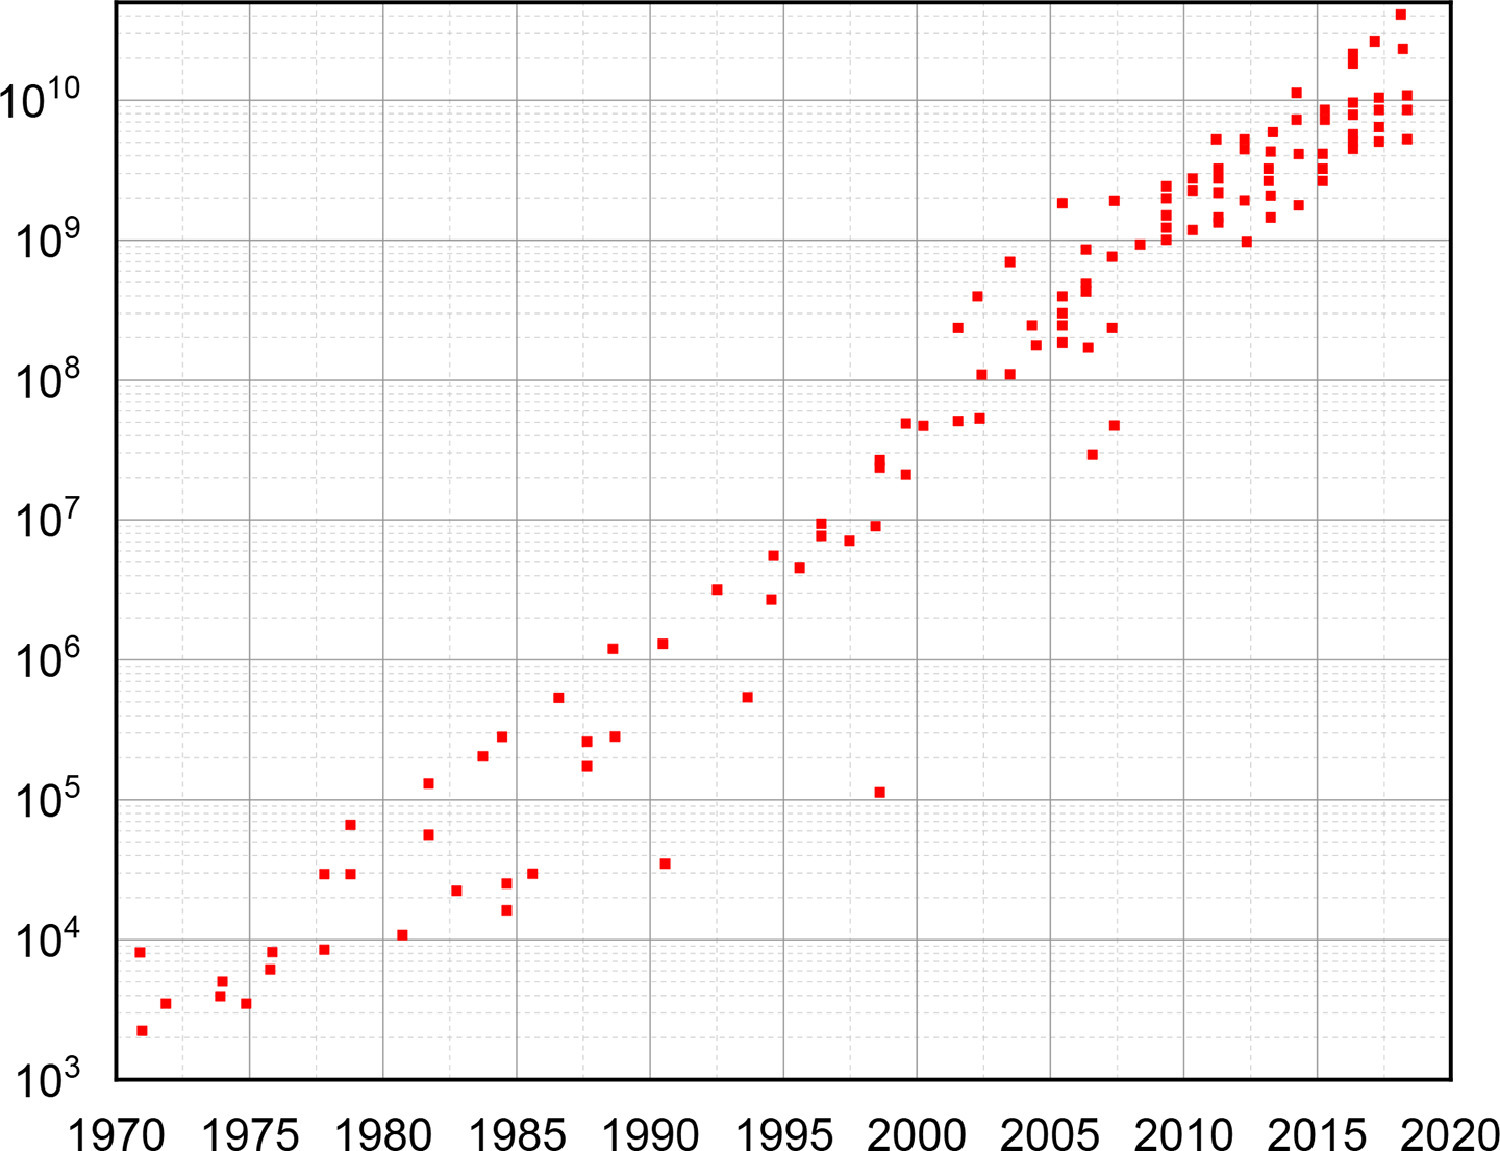
\includegraphics[width =0.5\linewidth]{chip-develop.jpg}
        \caption{半导体芯片上的晶体管数量}
        \label{chip-develop}
        \end{figure}


    \begin{equation}
        MTF = \frac{1}{{A{J^2}}}{\rm{exp}} - \frac{\phi }{{{K_B}T}}
        \label{MTF}
        \end{equation}



本论文以时域积分方程时间步进算法的数值实现技术、后时稳定性问题以及两层平面波加速算法为重点研究内容,主要创新点与贡献如下:

        \begin{algorithm}[H]
            \KwData{this text}
            \KwResult{how to write algorithm with \LaTeX2e}
            initialization\;
            \While{not at end of this document}{
                read current\;
                \eIf{understand}{
                    go to next section\;
                    current section becomes this one\;
                }{
                    go back to the beginning of current section\;
                }
            }
            \caption{How to wirte an algorithm.}
        \end{algorithm}


    % % !Mode:: "TeX:UTF-8"
%此为章节二模板
%\chapter、\section、\subsection、\subsubsection分别对应一二三四级标题
\chapter{相关理论基础及散热结构设计方案}\label{ch:2}

\section{表格示例}
可使用excel绘制表格,然后粘贴到以下网站中生成latex表格代码。

推荐网站如下:
https://www.tablesgenerator.com/

https://www.latex-tables.com/

\subsection{普通三线表示例}
普遍学者认为,微通道指的是水力直径在 $10\ \rm{\mu m}$ 到 $1000\ \rm{\mu m}$ 范围内的通道(也有观点认为是 $1\ \rm{\mu m}$ 到 $100\ \rm{\mu m}$)所构成的换热器。
以下是较为常见的微通道尺寸分类,可以参见\cref{tab:division-of-microchannels}。
\begin{table}[htbp]
    \caption[微通道的划分]{微通道的划分\cite{LuSiHong_2021}}
    \setlength{\tabcolsep}{14mm}{ % 因表格过窄,手动设置宽度为7mm
        \begin{tabular}{lc}
            \toprule
            通道种类    & 水力直径$\mu m$   \\
            \midrule
            分子纳米通道  & $\le 0.1$     \\
            过渡性纳米通道 & $0.1\sim 1$   \\
            过渡性微通道  & $1\sim 10$    \\
            微通道     & $10\sim 1000$ \\
            常规通道    & $>1000$       \\
            \bottomrule
        \end{tabular}}
    \label{tab:division-of-microchannels}
\end{table}



\subsection{跨页表格示例}

\begin{longtable}{@{\extracolsep{\fill}}cccccc@{}}  \\
    \caption{RSM仿真实验规划表}
    \label{tab:Experimental-Planning}  \\
    \toprule
    标准序 & 运行序 & $H_{rib}\ \rm{(mm)}$ & $H_{pf}\ \rm{(mm)}$ & $N_{pf}$ & $N_{ac}$ \\ \midrule
    \endfirsthead
    %
    \multicolumn{6}{c}%
    {{表 \thetable\ RSM仿真实验规划表 (续)}} \\
    \toprule
    标准序 & 运行序 & $H_{rib}\ \rm{(mm)}$ & $H_{pf}\ \rm{(mm)}$ & $N_{pf}$ & $N_{ac}$ \\ \midrule
    \endhead
    %
    \bottomrule
    \endfoot
    %
    \endlastfoot
    %
    11  & 1   & 0.16            & 0.8            & 6        & 16       \\
    13  & 2   & 0.16            & 0.16           & 22       & 16       \\
    15  & 3   & 0.16            & 0.8            & 22       & 16       \\
    12  & 4   & 0.8             & 0.8            & 6        & 16       \\
    10  & 5   & 0.8             & 0.16           & 6        & 16       \\
    2   & 6   & 0.8             & 0.16           & 6        & 0        \\
    19  & 7   & 0.48            & 0.48           & 14       & 8        \\
    1   & 8   & 0.16            & 0.16           & 6        & 0        \\
    20  & 9   & 0.48            & 0.48           & 14       & 8        \\
    18  & 10  & 0.48            & 0.48           & 14       & 8        \\
    8   & 11  & 0.8             & 0.8            & 22       & 0        \\
    14  & 12  & 0.8             & 0.16           & 22       & 16       \\
    6   & 13  & 0.8             & 0.16           & 22       & 0        \\
    17  & 14  & 0.48            & 0.48           & 14       & 8        \\
    7   & 15  & 0.16            & 0.8            & 22       & 0        \\
    16  & 16  & 0.8             & 0.8            & 22       & 16       \\
    4   & 17  & 0.8             & 0.8            & 6        & 0        \\
    9   & 18  & 0.16            & 0.16           & 6        & 16       \\
    5   & 19  & 0.16            & 0.16           & 22       & 0        \\
    3   & 20  & 0.16            & 0.8            & 6        & 0        \\
    25  & 21  & 0.48            & 0.48           & 6        & 8        \\
    22  & 22  & 0.8             & 0.48           & 14       & 8        \\
    23  & 23  & 0.48            & 0.16           & 14       & 8        \\
    29  & 24  & 0.48            & 0.48           & 14       & 8        \\
    28  & 25  & 0.48            & 0.48           & 14       & 16       \\
    30  & 26  & 0.48            & 0.48           & 14       & 8        \\
    26  & 27  & 0.48            & 0.48           & 22       & 8        \\
    27  & 28  & 0.48            & 0.48           & 14       & 0        \\
    21  & 29  & 0.16            & 0.48           & 14       & 8        \\
    24  & 30  & 0.48            & 0.8            & 14       & 8        \\ \bottomrule
\end{longtable}

\section{本章小节}
本章介绍了基于嵌入式散热模块的微通道散热技术所涉及的基……
    % % !Mode:: "TeX:UTF-8"

\chapter{基于嵌入式散热模块的微通道流动与传热性能研究}\label{ch:3}

\section{公式示例}
在本次研究中应用到计算流体动力学(Computational Fluid Dynamics,CFD)对研究对象进……。


\subsection{普通带序号公式}
\begin{equation}
    \frac{\partial u}{\partial x}+\frac{\partial v}{\partial y}+\frac{\partial v}{\partial z}=0
\end{equation}
u,v,w 分别是 x,y,z 方向的速度分量。


\subsection{需要对齐的多个带序号的公式}
\&号为对其对齐标记
\begin{align}% 式中的&为对齐的位置标记
    u & \frac{\partial u}{\partial x}+v \frac{\partial u}{\partial y}+w \frac{\partial u}{\partial z}=-\frac{1}{\rho_{f}} \frac{\partial p}{\partial x}+\frac{\mu_{f}}{\rho_{f}}\left(\frac{\partial^{2} u}{\partial x^{2}}+\frac{\partial^{2} u}{\partial y^{2}}+\frac{\partial^{2} u}{\partial z^{2}}\right) \\
    u & \frac{\partial v}{\partial x}+v \frac{\partial v}{\partial y}+w \frac{\partial v}{\partial z}=-\frac{1}{\rho_{f}} \frac{\partial p}{\partial y}+\frac{\mu_{f}}{\rho_{f}}\left(\frac{\partial^{2} v}{\partial x^{2}}+\frac{\partial^{2} v}{\partial y^{3}}+\frac{\partial^{2} v}{\partial z^{3}}\right) \\
    u & \frac{\partial w}{\partial x}+v \frac{\partial w}{\partial y}+w \frac{\partial w}{\partial z}=-\frac{1}{\rho_{f}} \frac{\partial p}{\partial z}+\frac{\mu_{f}}{\rho_{f}}\left(\frac{\partial^{2} w}{\partial x^{2}}+\frac{\partial^{2} w}{\partial y^{2}}+\frac{\partial^{2} w}{\partial z^{2}}\right)
\end{align}
$\rho_{f}$ 和 $\mu_{f}$ 分别是冷却剂的密度和动态粘度,p 是冷却剂压力。


\subsection{需要换行对齐的长公式}

\&号为对其对齐标记最好放置在计算符号之前,如=、+、-之前。
\backslash\backslash 表示换行。

\begin{equation}\label{eq:P}
    \begin{split}
        f_3 & = 6.272 + 3.02 H_{rib} + 6.08 H_{pf} + 0.0368 N_{pf} - 0.8848 N_{ac} + 0.04381 N_{ac}^2\\
        & + 6.35 H_{rib} \times H_{pf} - 0.3602 H_{rib}\times N_{ac} - 0.5497 H_{pf}\times N_{ac}
    \end{split}
\end{equation}

\subsection{其他公式示例}
\begin{equation}
    \begin{aligned}
    \left\{
        \begin{array}{l}
        \text {find}\enspace H_{rib},H_{rib},N_{pf},N_{ac} \\
        \text {min} \enspace F(H_{rib},H_{rib},N_{pf},N_{ac})= min\{f_1,f_2,f_3\} \\

            \text{s.t.\enspace}\enspace 0.2 \leqslant H_{rib} \leqslant 0.8                    \\
            \hspace{2.2em} 0.2 \leqslant H_{pf} \leqslant 0.8                     \\
            \hspace{2.2em} 6 \leqslant N_{pf} \leqslant 22,\ N_{pf}\in \mathbb{O} \\
            \hspace{2.2em} 0 \leqslant N_{ac} \leqslant 16,\ N_{ac}\in \mathbb{E}
        \end{array}
    \right. 
    \end{aligned}
    \label{eq:MO}
\end{equation}
    % % !Mode:: "TeX:UTF-8"

\chapter{基于嵌入式散热模块的微通道多目标结构优化}\label{ch:4}

\section{概述}
本章在\cref{ch:3}完成基……。

\section{列表示例}\label{sec:enumerate}

\subsection{普通列表示例}
\begin{enumerate}
    \item 在基板内部进行微通道散热以缩短传热路径,见\cref{fig:LTCC-Microchannels};
    \item 在基板内嵌入散热模块减少整体热阻,提高热传导效率,见\cref{fig:Embedded-cooling-module};
    \item 在嵌入式散热模块上制作针鳍或肋增强对流传热,以进一步减小热阻,见\cref{fig:Rib-pin-fin}。
\end{enumerate}

\subsection{标号为阿拉伯数字的列表}

\begin{enumerate}[label =(\arabic*)]

    \item 基于嵌入式散热模块的微通道流动与传热性能研究。
          将三种带有嵌入式散热模块的微通道:带有针鳍……
          最终选用MC-RPF作为核心散热结构;
    \item 分析几何参数对带有针鳍-肋嵌入式散热模块微通道流动与传热的影响。
          主要研究……;
    \item 对采用针鳍-肋嵌入式散热模块的微通道进行多目标优化。
          采用响应面分析法(Response Surface Methodology,RSM)与……;
    \item 基于MC-RPF的多热源散热结构设计分析。
          为解决在多热源应……;
    \item 基于MC-RPF的多热源散热结构压降优化。
          以压降损失相关理论为指导依据,……。

\end{enumerate}

\subsection{自定义列表标号}
\noindent NSGA-Ⅱ具体操作步骤如下:
\begin{enumerate}[leftmargin = 6em, labelsep = 0em]
    \item[步骤一、] 随机生成初始化种群,设置代数$Gen = 0$;
    \item[步骤二、] 判断是否生成第一代种群,如已生成则令其代数$Gen = 2$,否则进行快速非支配排序、选择、SBX、PM生成第一代子群,并设置代数$Gen = 2$;
    \item[步骤三、] 将父代与子代的种群进行合并形成新的父代种群;
    \item[步骤四、] 判断是否生成新的父代种群,如果未生成则进行快速非支配排序、拥挤度计算、精英策略选择操作以生成新的父代;
    \item[步骤五、] 对新生成的父代进行选择、SBX、PM操作生成新子群;
    \item[步骤六、] 判断当前代数是否小于设置的最大代数,若小于设置的最大代数则返回步骤三进行循环,否则,NSGA-Ⅱ结束运行。
\end{enumerate}

\section{本章小节}
    % % !Mode:: "TeX:UTF-8"

\chapter{基于MC-RPF的多热源散热结构设计分析及压降优化}\label{ch:5}

\section{算法示例}

\noindent 算法示例如下:

\begin{algorithm}[H]
    \KwData{this text}
    \KwResult{how to write algorithm with \LaTeX2e}
    initialization\;
    \While{not at end of this document}{
        read current\;
        \eIf{understand}{
            go to next section\;
            current section becomes this one\;
        }{
            go back to the beginning of current section\;
        }
    }
    \caption{How to wirte an algorithm.}
\end{algorithm}


\section{定理定义的使用示例}
\begin{theorem}
如果时域混合场积分方程是时域电场积分方程与时域磁场积分方程的线性组合。
\end{theorem}
\begin{proof}
由于时域混合场积分方程是时域电场积分方程与时域磁场积分方程的线性组合,因此时域混合场积分方程时间步进算法的阻抗矩阵特征与时域电场积分方程时间步进算法的阻抗矩阵特征相同。
\end{proof}
\begin{corollary}
时域积分方程方法的研究近几年发展迅速,在本文研究工作的基础上,仍有以下方向值得进一步研究。
\end{corollary}
\begin{lemma}
因此时域混合场积分方程时间步进算法的阻抗矩阵特征与时域电场积分方程时间步进算法的阻抗矩阵特征相同。
\end{lemma}
    % % !Mode:: "TeX:UTF-8"

\chapter{全文总结与展望}\label{ch:6}

\section{全文总结}
\section{空白符号}
    % 空行分段,多个空行等同于一个
    % 自动缩进,绝对不能使用空行代替
    % 英文中多个空格处理为一个空格,中文中空格会被忽略
    % 汉字与其他字符的间距会自动有XeLaTeX处理
    % 禁止使用中文全角空格
 
    % 1em(当前字体中M的宽度)
    1em: a\quad b
 
    % 2em
    2em: a\qquad b
 
    % 约为1/6个em
    1/6个em: a\,b 或 a\thinspace b
 
    % 0.5个em
    0.5个em: a\enspace b
 
    % 空格
    空格: a\ b
 
    % 硬空格,即不能分割的空格
    硬空格: a~b
 
    % 1pc=12pt=4.218mm
    指定宽度1pc: a\kern 1pc b
 
    指定宽度-1em: a\kern -1em b
 
    指定宽度1em: a\hskip 1em b
 
    指定宽度35pt: a\hspace{35pt}b
 
    % 占位宽度
    占位宽度为xyz: a\hphantom{xyz}b
 
    % 弹性长度hfill命令用于撑满整个空间
    弹性长度: a\hfill b

\section{\LaTeX 控制符}
\#              % 输出井号
\$              % 输出美元符号
\{ \}           % 输出大括号
\~{}            % 输出波浪
\_{}            % 输出下划线
\^{}            % 输出尖角
\textbackslash  % 输出反斜杠
\&              % 输出与符号


\section{后续工作展望}

    % \thesisbibliography{./reference/reference.bib} % 默认调用thesis-guet参考文献样式,当参考文献数目超过100时,可以使用large选项调整编号
    % % \bibliographystyle{thesis-guet(base-gbt7714-numerical)} % 参考文献样式
    % % \bibliography{reference} % 参考文献库
    % \thesisacknowledgement % 致谢
    % \thesisaccomplish % 攻读专业硕士学位期间取得的成果

    
\end{document}
